%%%%%%%%%%%%%%%%%%%%%%%%%%%%%%%%%%%%%%%%%
% "ModernCV" CV and Cover Letter
% LaTeX Template
% Version 1.2 (25/3/16)
%
% This template has been downloaded from:
% http://www.LaTeXTemplates.com
%
% Original author:
% Xavier Danaux (xdanaux@gmail.com) with modifications by:
% Vel (vel@latextemplates.com)
%
% License:
% CC BY-NC-SA 3.0 (http://creativecommons.org/licenses/by-nc-sa/3.0/)
%
% Important note:
% This template requires the moderncv.cls and .sty files to be in the same 
% directory as this .tex file. These files provide the resume style and themes 
% used for structuring the document.
%
%%%%%%%%%%%%%%%%%%%%%%%%%%%%%%%%%%%%%%%%%

%----------------------------------------------------------------------------------------
%	PACKAGES AND OTHER DOCUMENT CONFIGURATIONS
%----------------------------------------------------------------------------------------

\documentclass[11pt,a4paper,sans]{moderncv} % Font sizes: 10, 11, or 12; paper sizes: a4paper, letterpaper, a5paper, legalpaper, executivepaper or landscape; font families: sans or roman

\moderncvstyle{casual} % CV theme - options include: 'casual' (default), 'classic', 'oldstyle' and 'banking'
\moderncvcolor{blue} % CV color - options include: 'blue' (default), 'orange', 'green', 'red', 'purple', 'grey' and 'black'

\usepackage{lipsum} % Used for inserting dummy 'Lorem ipsum' text into the template
\usepackage{pdfpages}

\usepackage[scale=0.75]{geometry} % Reduce document margins
%\setlength{\hintscolumnwidth}{3cm} % Uncomment to change the width of the dates column
%\setlength{\makecvtitlenamewidth}{10cm} % For the 'classic' style, uncomment to adjust the width of the space allocated to your name

%----------------------------------------------------------------------------------------
%	NAME AND CONTACT INFORMATION SECTION
%----------------------------------------------------------------------------------------

\firstname{Lars} % Your first name
\familyname{Hjerrild} % Your last name

% All information in this block is optional, comment out any lines you don't need
\title{CV}
\address{Jens Baggesensvej 118, 8200}{Aarhus N, Danmark}
\mobile{(+45) 42 42 08 83}
\phone{(None) }
%\fax{(000) 111 1113}
\email{larshjerrild@hotmail.com}
%\homepage{staff.org.edu/~jsmith}{staff.org.edu/$\sim$jsmith} % The first argument is the url for the clickable link, the second argument is the url displayed in the template - this allows special characters to be displayed such as the tilde in this example
%\extrainfo{additional information}
\photo[90pt][0.4pt]{pictures/picture} % The first bracket is the picture height, the second is the thickness of the frame around the picture (0pt for no frame)
%\quote{"T" - John Smith}

%----------------------------------------------------------------------------------------

\begin{document}

%----------------------------------------------------------------------------------------
%	COVER LETTER
%----------------------------------------------------------------------------------------

% To remove the cover letter, comment out this entire block

%\clearpage
%
%\recipient{HR Department}{Corporation\\123 Pleasant Lane\\12345 City, State} % Letter recipient
%\date{\today} % Letter date
%\opening{Dear Sir or Madam,} % Opening greeting
%\closing{Sincerely yours,} % Closing phrase
%\enclosure[Attached]{curriculum vit\ae{}} % List of enclosed documents
%
%\makelettertitle % Print letter title
%
%\lipsum[1-3] % Dummy text
%
%\makeletterclosing % Print letter signature
%

\textbf{Ans\o gning  vedr. stillingen "Praktik: Softwareudvikler" ved Systematic}
\vspace{2mm} 
\\
 Stillingsopslaget lyder sp\ae ndende af flere \aa rsager, men appellere prim\ae rt til mig pga. systematics store fokus p{\aa} process, der g\o r at de kan tilbyde noget der ikke findes andetsteds. St\o rrelsen af virksomhedens produkter kr\ae ver ogs{\aa} at software arktitekturen skal v\ae re gennemt\ae nkt og det synes jeg er sp\ae ndende. \\

Jeg mener jeg er den rigtige til stillingen, fordi jeg er velovervejet og g\aa r op i at det software jeg udvikler skal v\ae re b\aa de vedligholdelses venligt og nemt at udvikle p\aa. Derigennem tror jeg p{\aa} at man f\aa r de bedste produkter. 
Desuden t\ae nker jeg meget over hvordan jeg arbejder og pr\o ver struktureret at komme til at arbejde bedre og mere effektivt. Jeg har tidligere selv deltaget i et scrum kursus udbudt af Systematic, og har derigennem f\aa et indtroduceret jeres arbejdsmetoder, og jeg vil gerne arbejde et sted hvor jeg kan v\ae re med til at effektificere udviklingsprocessen, som en del af udviklingsteamet.\\



Jeg kunne godt t\ae nke mig at arbejde med backend-udviklingen som b\aa de indeholder uafh\ae ngige applikationer, men ogs\aa selve informationsstyringen synes jeg lyder sp\ae ndende. Jeg kan godt noget front-end udvikling, men synes ikke det er lige s{\aa} sp\ae ndende.

Generelt synes jeg at afdelingerne Health og Defence lyder mest attraktive for mig, simpelthen da jeg synes at dom\ae net er sjovt.\\

Personligt er jeg en nem person der godt kan lide at lave mange forskellige ting. Fx spiller jeg musik, har l\o bet en del igennem tiden, og er med i en hockey forening hvor jeg spiller en gang om ugen. Se mere under CV.\\ 








\vspace{3mm}
Med venlig hilsen

\vspace{5mm}
Lars Hjerrild



\vspace{10mm}
%Bilag : CV og Karakterudskrift 







\newpage

%----------------------------------------------------------------------------------------
%	CURRICULUM VITAE
%----------------------------------------------------------------------------------------

\makecvtitle % Print the CV title

%----------------------------------------------------------------------------------------
%	EDUCATION SECTION
%----------------------------------------------------------------------------------------

\section{Om mig}
Personligt kan jeg godt lide at v\ae re aktiv og bruger tid p{\aa} at tr\ae ne og elsker at komme udenfor. Jeg spiller fast hockey et par timer om ugen, og har som teenager (15-20) g\aa et rigtig meget op i orienteringsl\o b, hvor jeg i fire \aa r var en del af det danske juniorlandshold. Jeg har derigennem l\ae rt  at arbejde struktureret p{\aa} at blive bedre, og hvor stor en betydning det milj\o man arbejder i har. Som person er jeg en smule stille, men jeg g\aa r meget op i at folk har det godt. Min gamle juniorlandstr\ae ner sagde til mig da jeg stoppede at han aldrig har haft en l\oe ber der havde givet ham s\aa mange high fives, hvilket jeg synes var meget sigende om mig. Jeg har interesse i musik og elsker at rejse. Jeg har s\aa gar boet i USA i et \aa r, og g\aa et p{\aa} en amerikansk elementary school s\aa selvom det ikke bliver brugt s\aa ofte l\ae ngere er mit engelsk stadig ganske godt. 

\section{Uddannelse}

\cventry{2015--2018}{DiplomIngeni\o r i information og kommunikationsteknologi}{Aarhus Universitet}{IHA}
{}{}  % Arguments not required can be left empty
\cventry{2010--2014}{STX}{Marselisborg Gymnasium}{}
{}{}
\cventry{2009--2010}{Efterskole}{himmelbjergegnens natur og idr\ae tsefterskole}{}
{}{}

%\section{Masters Thesis}
%\cvitem{Title}{\emph{Money Is The Root Of All Evil -- Or Is It?}}
%\cvitem{Supervisors}{Professor James Smith \& Associate Professor Jane Smith}
%\cvitem{Description}{This thesis explored the idea that money has been the cause of untold anguish and suffering in the world. I found that it has, in fact, not.}


%----------------------------------------------------------------------------------------
%	WORK EXPERIENCE SECTION
%----------------------------------------------------------------------------------------

\section{Erfaring}

Arbejdede i en ganske kort periode som vikar, hvor jeg hjalp som lagerarbejder. Det hjalp til at sparre op til at komme ud og rejse. 
%
%\subsection{Vocational}
%
%\cventry{2012--Present}{1\textsuperscript{st} Year Analyst}{\textsc{Lehman Brothers}}{Los Angeles}{}{Developed spreadsheets for risk analysis on exotic derivatives on a wide array of commodities (ags, oils, precious and base metals), managed blotter and secondary trades on structured notes, liaised with Middle Office, Sales and Structuring for bookkeeping.
%\newline{}\newline{}
%Detailed achievements:
%\begin{itemize}
%\item Learned how to make amazing coffee
%\item Finally determined the reason for \textsc{PC LOAD LETTER}:
%\begin{itemize}
%\item Paper jam
%\item Software issues:
%\begin{itemize}
%\item Word not sending the correct data to printer
%\item Windows trying to print in letter format
%\end{itemize}
%\item Coffee spilled inside printer
%\end{itemize}
%\item Broke the office record for number of kitten pictures in cubicle
%\end{itemize}}

%------------------------------------------------

%\cventry{2010--2011}{Summer Intern}{\textsc{Lehman Brothers}}{Los Angeles}{}{Rated "truly distinctive" for Analytical Skills and Teamwork.}

%------------------------------------------------
%


Jeg har efterh\aa nden mange gange arrangeret l\o b og tr\ae ning hvor jeg uden fastans\ae ttelse har tjent penge b\aa de til mig selv eller til min egen klub(Orienteringsl\o b).

%
%\cventry{2008--2009}{Computer Repair Specialist}{Buy More}{Burbank}{}{Worked in the Nerd Herd and helped to solve computer problems by asking customers to turn their computers off and on again.}

%----------------------------------------------------------------------------------------
%	AWARDS SECTION
%----------------------------------------------------------------------------------------
%
%\section{Om mig}
%
%\cvitem{2011}{School of Business Postgraduate Scholarship}
%\cvitem{2010}{Top Achiever Award -- Commerce}

%----------------------------------------------------------------------------------------
%	COMPUTER SKILLS SECTION
%----------------------------------------------------------------------------------------

\section{Faglig kompetancer}

\cvitem{}{\textsc{C}    \textsc{C++}  \textsc{C\#} \textsc{WPF} \textsc{Entity-Framework}}
\cvitem{}{\textsc{Bootstrap} \textsc{CSS3}   \textsc{HTML5} \textsc{ASP.Net}  }
\cvitem{}{\textsc{Scrum} \textsc{Projektarbejde} \textsc{Git} \textsc{Linux} \textsc{NUnit}}

%----------------------------------------------------------------------------------------
%	COMMUNICATION SKILLS SECTION
%----------------------------------------------------------------------------------------
%
%\section{Communication Skills}
%
%\cvitem{2010}{Oral Presentation at the California Business Conference}
%\cvitem{2009}{Poster at the Annual Business Conference in Oregon}

%----------------------------------------------------------------------------------------
%	LANGUAGES SECTION
%----------------------------------------------------------------------------------------

%----------------------------------------------------------------------------------------
%	INTERESTS SECTION
%----------------------------------------------------------------------------------------

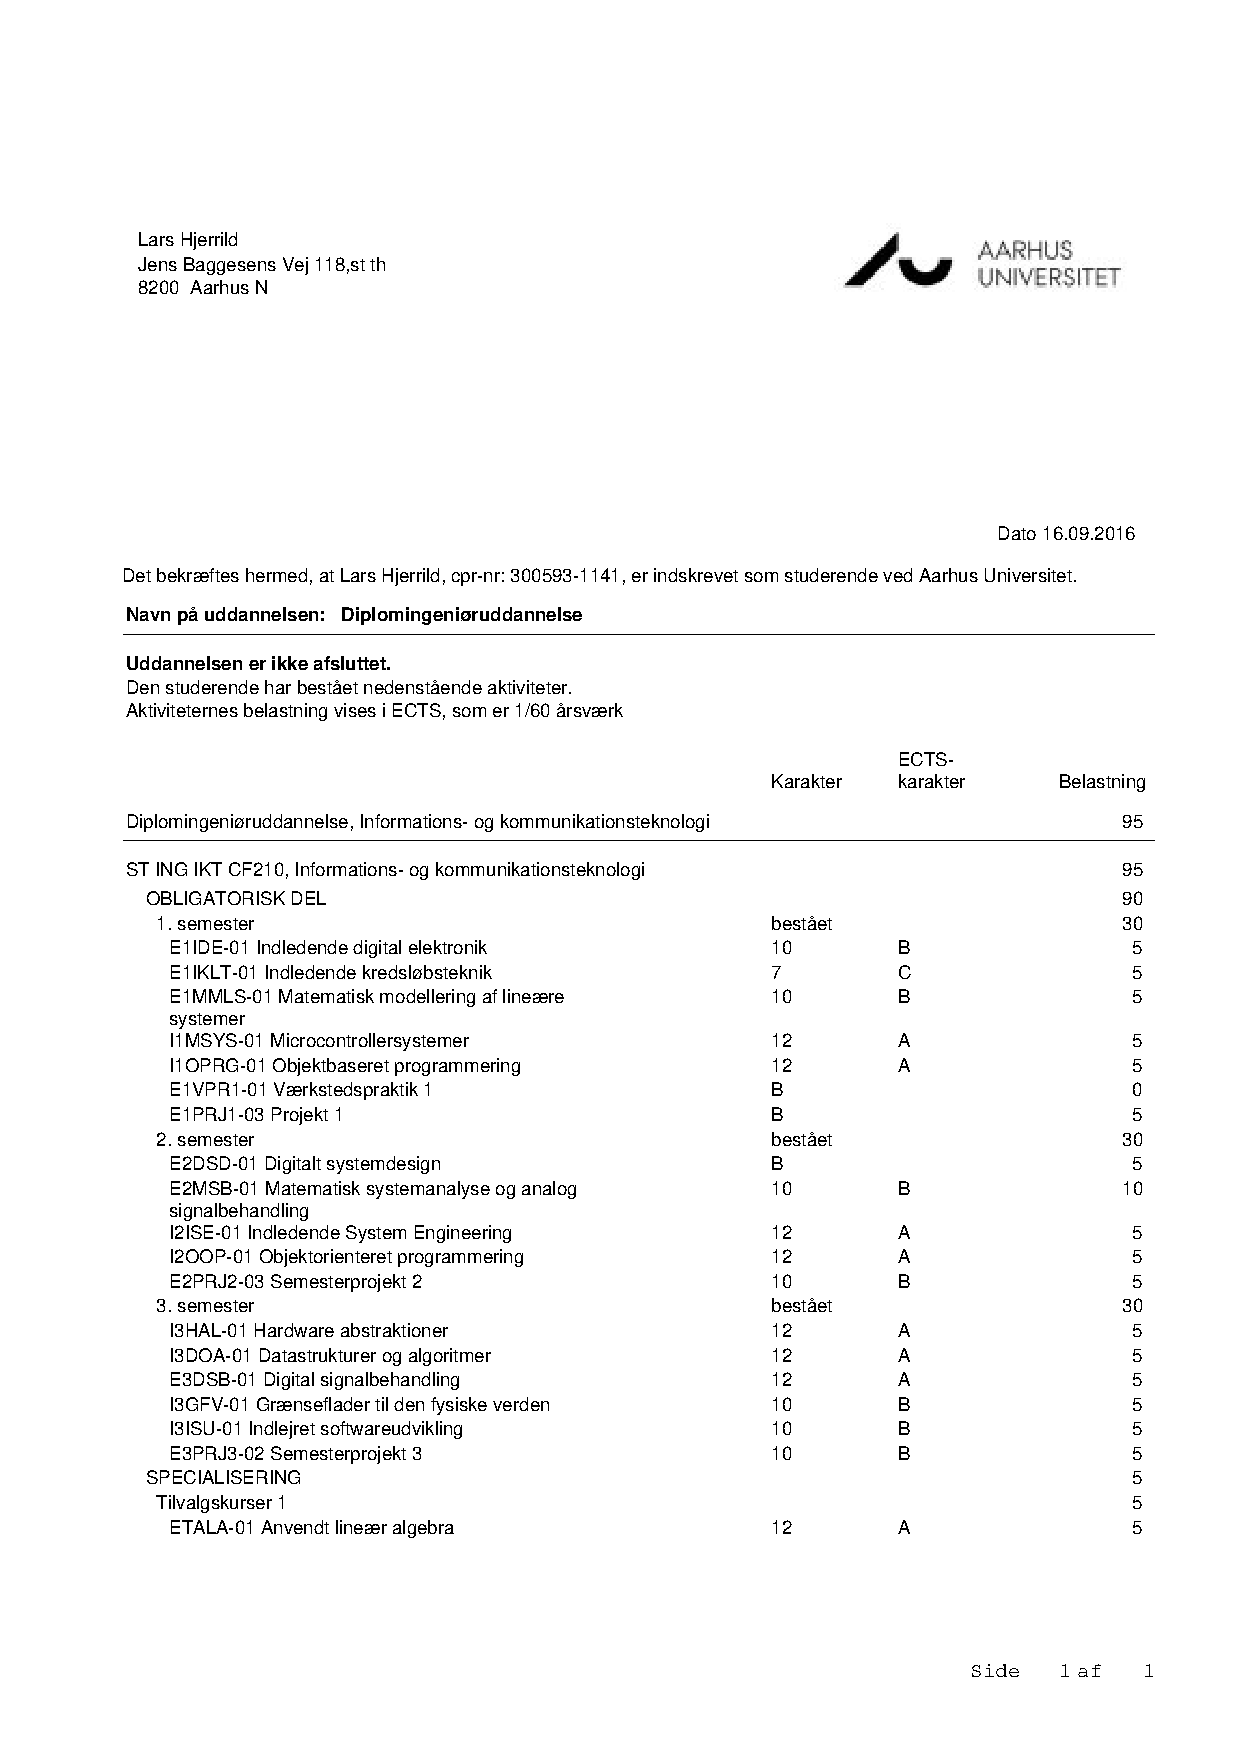
\includepdf[pages={1}]{pictures/Karakterudskrift.pdf}

%----------------------------------------------------------------------------------------

\end{document}